\documentclass[i1]{oss}
\setlength{\topmargin}{-.5in}
\setlength{\textheight}{9in}
\setlength{\oddsidemargin}{.100in}
\setlength{\textwidth}{6.25in}
\usepackage [dutch] {babel}
\usepackage{graphicx}
\usepackage{amsmath}
\usepackage{fullpage}
\usepackage{color}
\usepackage{soul}
\usepackage{gensymb}
\usepackage{caption}
\usepackage{subcaption}
\usepackage[section]{placeins}

\begin{document}

\members{Joren Verspeurt {\small \texttt{(r0258417)} } \\
         Sophie Marien {\small \texttt{(s0216517)}}\\
         Stef Noten {\small \texttt{(s0211264)}}\\
         Toon Nolten {\small \texttt{(r0258654)}} \\
         Begeleider: Mario H. C. T.} % teamleden

\maketitlepage
\newpage
\tableofcontents
\pagebreak




%----------------------------------------------------------------------------------------
%	INLEIDING
%----------------------------------------------------------------------------------------
\section*{Inleiding}
\label{ssec:Inleiding}


%----------------------------------------------------------------------------------------
%	ONTWERP
%----------------------------------------------------------------------------------------
\section{Ontwerp}
\label{ssec:Ontwerp}
%Klassendiagram en interactie diagrammen



%-------------KLASSENDIAGRAMMA-------------------------------
\subsection{Klassendiagramma}
\label{ssec:Klassendiagramma}


%-------------Interactie Diagrammas-------------------------------
\subsection{Interactie diagrammas}
\label{ssec:Interactiedia}


%-------------Ontwerpbeslissingen-------------------------------
\subsection{Ontwerpbeslissingen en patronen}
\label{ssec:Ontwerpbeslissingen}



%----------------------------------------------------------------------------------------
%	TESTEN
%----------------------------------------------------------------------------------------
\section{Testen}
\label{ssec:testen}
%Een hoofdstuk rond testen dat de procedure beschrijft die gevolgd werd bij het testen: wat
%werd getest en hoe?


%----------------------------------------------------------------------------------------
%	PROJECT MANAGMENT
%----------------------------------------------------------------------------------------
\section{Project management}
\label{ssec:Projectmanag}
%taakverdeling elk lid en welke taak
%uren

%TODO tekst

%TODO laatste week aanvullen!!
\begin{table}[h!]
\begin{center}
    \begin{tabular}{ r | c  c  c  c  c  c}
     & Joren & Toon & Stef & Sophie \\ \hline
    Algemeen & 2u00 & 2u00 & 2u00 & 2u00\\
           Tools & 8u30 & 8u30 & 8u00 & 4u30 \\
        Analyse & 10u00 & 10u00 & 12u15 & 12u00 \\
        Ontwerp & 00u00 & 00u00 & 00u00 & 00u00 \\
        Implementeren & 00u00 & 00u00 & 00u00 & 00u00\\
        Verslag & 9u00 & 9u00 & 9u00 & 9u00 \\
        Totaal & 29u30 & 29u30 & 31u15 & 27u30  
    \end{tabular}
    \caption{Overzicht werkuren per onderdeel}
    \label{tab:werkuren}
\end{center}
\end{table}

%TODO figuren updaten
\begin{figure}[h!]
        \centering
        \begin{subfigure}[hb]{0.20\textwidth}
                \centering
                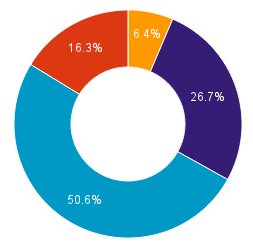
\includegraphics[width=\textwidth]{chart_2}
                \caption{Joren}
        \end{subfigure}%
        \begin{subfigure}[hb]{0.20\textwidth}
                \centering
                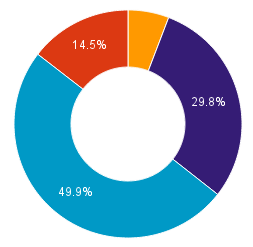
\includegraphics[width=\textwidth]{chart_3}
                \caption{Toon}
        \end{subfigure}%
        \begin{subfigure}[hb]{0.20\textwidth}
                \centering
                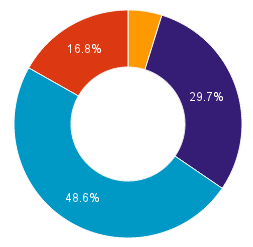
\includegraphics[width=\textwidth]{chart_4}
                \caption{Stef}
        \end{subfigure}%
        \begin{subfigure}[hb]{0.20\textwidth}
                \centering
                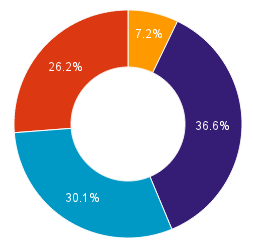
\includegraphics[width=\textwidth]{chart_5}
                \caption{Sophie}
        \end{subfigure}%
                \begin{subfigure}[hb]{0.20\textwidth}
                \centering
                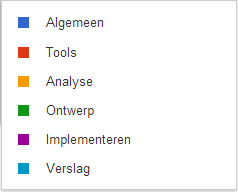
\includegraphics[width=\textwidth]{legende}
                \caption{Legende}
        \end{subfigure}%


 \caption{Weergave van de werkverdeling}
\label{fig:werkverdeling}
\end{figure}





%----------------------------------------------------------------------------------------
%	 CONCLUSIE en DISCUSSIE
%----------------------------------------------------------------------------------------
\section{Conclusie}
\label{ssec:Conclusie}
% Een hoofdstuk met een discussie en conclusie waarin interessante ervaringen, problemen en
%andere opmerkingen omtrent het project worden beschreven



%----------------------------------------------------------------------------------------
%	GLOSSARY
%----------------------------------------------------------------------------------------
\section{Glossary}
\label{ssec:glossary}


Daemon met een policy en een testinformation Klasse en een Statistic information 

Pattern Model-View-Controller
View:  GUI, CLI, passive view
Controller:
Input besturingsview, handeld input/output
Model: Daemon, Policy, TestInfomation, DataCollector, Statistic, TestRun
Daemon is bedoeld als interface voor het model

Verantwoordelijkheden
Policy: ordening, filtering
Statistic: berekent de statistieken, legt een strategie vast om data op te vragen.
TestInformation:  Houdt de statistieken bij (alles dat uit de collectors wordt opgevraagd)
DataCollector: Data verzameling, inpluggen in een TestRun, change code bijhouden (apart in een andere Collector)
Daemon:  Starten van TestRuns
TestRun:  runnen van testen

Implementaties:
Policy als Composit/Decorator/Strategy
We weten niet zeker of het een composit is want er werd getwijfeld tussen Composit en Decorator Pattern. 
Statistic en DataCollector zijn een Strategy
TestInfomation
Eerst mapte Description met een lijst van tuples. Dit is veranderd naar TestSummary
Map<Description,OrderedSet<TestSummary>>
	TestSummary	-Map<Collector, Object>
			- TestID


We streven voor low-coupling. Deamon weet alleen maar af van de actieve policies en de policies waarvoor hem op dat moment de statistieken gaat berekenen, de TestRuns en de TestInformation. Daemon weet wat hij moet weten en niet te veel. 

Verslag: beginnen met de analyse van wat we nodig hebben en daarna uitleggen hoe we dit oplossen en analyseren en bediscussiëren.

 


\end{document}



